%==========================================================================
%   PRESENTACIÓN DE DEFENSA DEL TFG - UC3M
%==========================================================================
%
%   Implementación en Julia de un elemento hexaédrico de Nédélec de
%   segundo orden para electromagnetismo computacional
%
%   Estructura basada en las diapositivas de Daniel Mohedano Rodríguez
%   ("Interoperability system between Julia and the electromagnetic
%   simulator HOFEM", Master's Thesis, UC3M, Septiembre 2025).
%
%   COMPILACIÓN:
%     pdflatex presentacion_tfg.tex
%     pdflatex presentacion_tfg.tex
%
%   NOTA: las figuras se referencian con rutas relativas a este archivo
%   (imagenes/ y figuras/). Compilar desde el directorio memoria/.
%==========================================================================

\documentclass[aspectratio=169,11pt]{beamer}

%----------
%	TEMA Y COLORES
%----------
\usetheme{Madrid}
\usecolortheme{default}

% Colores corporativos UC3M
\definecolor{azulUC3M}{RGB}{0,0,102}
\definecolor{grisUC3M}{RGB}{88,88,88}

\setbeamercolor{structure}{fg=azulUC3M}
\setbeamercolor{palette primary}{bg=azulUC3M,fg=white}
\setbeamercolor{palette secondary}{bg=azulUC3M,fg=white}
\setbeamercolor{palette tertiary}{bg=azulUC3M,fg=white}
\setbeamercolor{frametitle}{bg=azulUC3M,fg=white}
\setbeamercolor{title}{fg=azulUC3M}
\setbeamercolor{author}{fg=grisUC3M}
\setbeamercolor{date}{fg=grisUC3M}

%----------
%	PAQUETES
%----------
\usepackage[utf8]{inputenc}
\usepackage[T1]{fontenc}
\usepackage[spanish]{babel}
\usepackage{amsmath,amssymb}
\usepackage{booktabs}
\usepackage{graphicx}
\usepackage{listings}
\usepackage{tikz}
\usetikzlibrary{arrows.meta,positioning,shapes.geometric}

%----------
%	LISTADOS DE CÓDIGO
%----------
% Definición del lenguaje Julia para listings (no viene de serie)
\lstdefinelanguage{Julia}{
  morekeywords={using,function,end,if,else,elseif,for,while,return,
                struct,mutable,module,import,export,const,let,do,
                true,false,nothing,in,where},
  sensitive=true,
  morecomment=[l]{\#},
  morecomment=[s]{\#=}{=\#},
  morestring=[b]",
  morestring=[b]',
}

\lstset{
  basicstyle=\ttfamily\scriptsize,
  keywordstyle=\color{azulUC3M}\bfseries,
  commentstyle=\color{grisUC3M}\itshape,
  stringstyle=\color{teal},
  showstringspaces=false,
  frame=single,
  rulecolor=\color{grisUC3M},
  breaklines=true,
  columns=fullflexible
}

%----------
%	METADATOS
%----------
\title[Elemento de Nédélec en Julia]{Implementación en Julia de un elemento hexaédrico de Nédélec de segundo orden para electromagnetismo computacional}
\author[Nombre Apellidos]{Nombre Apellidos\\[2mm]\footnotesize Tutor: Nombre del tutor}
\institute[UC3M]{Universidad Carlos III de Madrid\\Grupo GREMA}
\date{\today}

% Logo en cada diapositiva (si existe el archivo)
\IfFileExists{imagenes/Portada_Logo.png}{%
  \logo{
\includegraphics[height=0.7cm]{imagenes/Portada_Logo.png}}%
}{}

%==========================================================================
\begin{document}
%==========================================================================

%--------------------------------------------------------------------------
% DIAPOSITIVA 1 — PORTADA
%--------------------------------------------------------------------------
\begin{frame}
  \titlepage
\end{frame}

%--------------------------------------------------------------------------
% DIAPOSITIVA 2 — ÍNDICE
%--------------------------------------------------------------------------
\begin{frame}{Índice}
  \tableofcontents
\end{frame}

%==========================================================================
\section{Motivación}
%==========================================================================

%--------------------------------------------------------------------------
% DIAPOSITIVA 3 — EL PROBLEMA DE LOS DOS LENGUAJES
%--------------------------------------------------------------------------
\begin{frame}{El problema de los dos lenguajes}
  \begin{itemize}
    \item Los lenguajes de alto nivel se agrupan en dos categorías:
      \begin{itemize}
        \item Lenguajes de sistema (rendimiento, compilados)
        \item Lenguajes de scripting (flexibilidad, interpretados)
      \end{itemize}
    \item En computación científica predomina el uso combinado:
      \begin{itemize}
        \item Prototipado rápido en lenguajes de scripting
        \item Implementación final en lenguajes de sistema
      \end{itemize}
    \item \alert{Consecuencia}: duplicación de código y barrera entre
          investigación y producción.
  \end{itemize}
\end{frame}

%--------------------------------------------------------------------------
% DIAPOSITIVA 4 — EL SIMULADOR HOFEM
%--------------------------------------------------------------------------
\begin{frame}{HOFEM}
  \begin{itemize}
    \item Simulador electromagnético paralelo desarrollado en GREMA
    \item Método de elementos finitos de alto orden (High Order FEM)
    \item Implementado en Fortran moderno
    \item Ejecución secuencial y paralela (MPI + OpenMP)
  \end{itemize}
\end{frame}

%--------------------------------------------------------------------------
% DIAPOSITIVA 5 — FORMULACIÓN Y FLUJO DE HOFEM
%--------------------------------------------------------------------------
\begin{frame}{Formulación de HOFEM}
  \textbf{Ecuación de onda curl-curl:}
  \begin{equation*}
    \nabla \times \left(f_r^{-1}\, \nabla \times \mathbf{V}\right)
    - k_0^2\, g_r\, \mathbf{V}
    = -j\, k_0\, h_0\, \mathbf{P}
    - \nabla \times \left(f_r^{-1}\, \mathbf{L}\right)
  \end{equation*}

  \textbf{Discretización:}
  \begin{equation*}
    [K]\{g\} = \{F\}, \qquad
    [K] = \sum [k^e], \qquad
    \{F\} = \sum \{f^e\}
  \end{equation*}

  \textbf{Flujo de simulación:}
  \begin{center}
    \footnotesize
    Configuración $\to$ Malla $\to$ Matrices de elemento $[k^e],\{f^e\}$
    $\to$ Ensamblado $[K],\{F\}$ $\to$ Solver disperso $\to$ Postproceso
  \end{center}
\end{frame}

%==========================================================================
\section{Visión general del proyecto}
%==========================================================================

%--------------------------------------------------------------------------
% DIAPOSITIVA 7 — OBJETIVOS PRINCIPALES
%--------------------------------------------------------------------------
\begin{frame}{Objetivos principales}
  \begin{enumerate}
    \item Implementar en Julia el elemento hexaédrico de Nédélec de segundo
          orden siguiendo la formulación de Amor-Martín y García-Castillo
          (IEEE TAP, 2023).
    \item Generar y verificar los coeficientes de las funciones de base
          (matriz $W$) reproduciendo la Tabla II del artículo de referencia.
    \item Validar mediante benchmarks analíticos: cavidad llena y cavidad
          semillena, comprobando el orden de convergencia teórico $O(h^4)$.
    \item Comparar el rendimiento en Julia frente a la implementación de
          referencia en MATLAB.
    \item Estructurar el código como paquete Julia modular, documentado y con
          suite de tests automatizados.
  \end{enumerate}
\end{frame}

%==========================================================================
\section{Arquitectura}
%==========================================================================

%--------------------------------------------------------------------------
% DIAPOSITIVA 9 — VISIÓN GENERAL
%--------------------------------------------------------------------------
\begin{frame}{Visión general}
  Sistema basado en dos componentes principales:

  \vspace{4mm}
  \begin{columns}[T]
    \begin{column}{0.48\textwidth}
      \begin{block}{Núcleo matemático}
        \begin{itemize}
          \item Bases
          \item Grados de libertad
          \item Transformaciones
        \end{itemize}
      \end{block}
    \end{column}
    \begin{column}{0.48\textwidth}
      \begin{block}{Ensamblado y resolución}
        \begin{itemize}
          \item Matrices globales
          \item Solver
          \item Benchmarks
        \end{itemize}
      \end{block}
    \end{column}
  \end{columns}

  \vspace{4mm}
  \begin{center}
    \footnotesize\itshape
    Diagrama de módulos del paquete NedelecHex
  \end{center}
\end{frame}

%--------------------------------------------------------------------------
% DIAPOSITIVA 10 — NÚCLEO MATEMÁTICO
%--------------------------------------------------------------------------
\begin{frame}{Núcleo matemático}
  \begin{itemize}
    \item Elemento de referencia: hexaedro unidad $[0,1]^3$
    \item Espacio mixto de orden 2:
      \begin{equation*}
        H_2 = Q_{1,2,2} \times Q_{2,1,2} \times Q_{2,2,1}
        \qquad (54 \text{ monomios})
      \end{equation*}
    \item 54 grados de libertad:
      \begin{itemize}
        \item 24 en aristas
        \item 24 en caras
        \item 6 en volumen
      \end{itemize}
    \item Generación de coeficientes: $G \cdot W = I \;\Rightarrow\; W = G^{-1}$
    \item Transformaciones de Piola covariante/contravariante
  \end{itemize}
\end{frame}

%--------------------------------------------------------------------------
% DIAPOSITIVA 11 — DEPENDENCIAS Y HERRAMIENTAS
%--------------------------------------------------------------------------
\begin{frame}{Dependencias y herramientas}
  \begin{itemize}
    \item \textbf{Julia} (JIT vía LLVM)
    \item \textbf{Gmsh}: generación de mallas hexaédricas
    \item \textbf{LinearAlgebra / SparseArrays}: álgebra lineal dispersa
    \item \textbf{Arpack}: resolución de autovalores (shift-invert)
    \item \textbf{MATLAB}: implementación de referencia para comparación
    \item \textbf{Manim}: visualizaciones explicativas
  \end{itemize}
\end{frame}

%--------------------------------------------------------------------------
% DIAPOSITIVA 12 — FLUJO DE TRABAJO
%--------------------------------------------------------------------------
\begin{frame}{Flujo de trabajo}
  \begin{center}
  \begin{tikzpicture}[
      node distance=2.5mm,
      every node/.style={
        draw, rounded corners, fill=azulUC3M!8, draw=azulUC3M,
        font=\tiny, align=center, inner sep=2pt,
        minimum height=5mm, text width=4.4cm
      },
      arrow/.style={-{Latex[length=1.6mm]}, draw=azulUC3M, thick}
    ]
    \node (mesh) {Malla Gmsh (\texttt{.msh})};
    \node (perm) [below=of mesh] {Lectura y permutación de nodos\\ \texttt{[3,7,8,4,2,6,5,1]}};
    \node (elem) [below=of perm] {Cálculo de matrices elementales\\ $[k^e], [m^e]$};
    \node (glob) [below=of elem] {Ensamblado global $[K], [M]$};
    \node (dir)  [below=of glob] {Aplicación de Dirichlet (PEC)};
    \node (solv) [below=of dir]  {Solver de autovalores};
    \node (post) [below=of solv] {Postproceso / comparación\\ con solución analítica};

    \foreach \a/\b in {mesh/perm, perm/elem, elem/glob, glob/dir, dir/solv, solv/post}
      \draw[arrow] (\a) -- (\b);
  \end{tikzpicture}
  \end{center}
\end{frame}

%==========================================================================
\section{Implementación}
%==========================================================================

%--------------------------------------------------------------------------
% DIAPOSITIVA 14 — GENERACIÓN DE COEFICIENTES
%--------------------------------------------------------------------------
\begin{frame}[fragile]{Generación de coeficientes}
  \begin{itemize}
    \item Construcción de la matriz de momentos $G$ ($54 \times 54$)
    \item Inversión: $W = G^{-1}$
    \item Verificación: $W$ coincide con la Tabla II del artículo
          (2916 entradas)
    \item Coeficientes enteros $\Rightarrow$ estabilidad numérica
  \end{itemize}

  \vspace{2mm}
  \begin{lstlisting}[language=Julia]
# CoefficientGenerator.jl
G = build_moment_matrix(order)
W = inv(G)              # 54x54, entradas enteras
@assert W == tabla_II   # verificacion exacta
  \end{lstlisting}
\end{frame}

%--------------------------------------------------------------------------
% DIAPOSITIVA 15 — EVALUACIÓN DE BASES
%--------------------------------------------------------------------------
\begin{frame}[fragile]{Evaluación de las funciones de base}
  \begin{itemize}
    \item Evaluación en el elemento de referencia
    \item Transformación al elemento real (Piola)
    \item Cálculo de Jacobiano y su inverso
    \item Vectorización para rendimiento
  \end{itemize}

  \vspace{2mm}
  \begin{lstlisting}[language=Julia]
# BasisEval.jl
N_ref = eval_basis_ref(xi, eta, zeta, W)
J     = jacobian(mesh, elem)
N     = piola_covariant(N_ref, J)   # elemento real
  \end{lstlisting}
\end{frame}

%--------------------------------------------------------------------------
% DIAPOSITIVA 16 — ENSAMBLADO Y CONDICIONES DE CONTORNO
%--------------------------------------------------------------------------
\begin{frame}{Ensamblado y condiciones de contorno}
  \begin{itemize}
    \item Numeración global de grados de libertad (aristas, caras, volumen)
    \item Ensamblado de $[K]$ y $[M]$ mediante cuadratura de Gauss-Legendre
    \item Aplicación de Dirichlet (PEC) por eliminación
    \item Uso de etiquetas de malla (PolyFace/Solid) en lugar de inferencia
          geométrica
  \end{itemize}
\end{frame}

%--------------------------------------------------------------------------
% DIAPOSITIVA 17 — RESOLUCIÓN DE AUTOVALORES
%--------------------------------------------------------------------------
\begin{frame}{Resolución del problema de autovalores}
  \begin{itemize}
    \item Problema generalizado:
      \begin{equation*}
        [K]\{g\} = \lambda\, [M]\{g\}
      \end{equation*}
    \item Método shift-invert con Arpack
    \item Solver denso para mallas pequeñas (verificación)
    \item Cálculo de la norma de energía para el análisis de error
  \end{itemize}
\end{frame}

%==========================================================================
\section{Validación}
%==========================================================================

%--------------------------------------------------------------------------
% DIAPOSITIVA 19 — SUITE DE TESTS
%--------------------------------------------------------------------------
\begin{frame}{Suite de tests}
  \begin{itemize}
    \item 11 ficheros de test que cubren todo el pipeline:
      \begin{itemize}
        \item Cuadratura, monomios, grados de libertad
        \item Coeficientes (comparación con Tabla II)
        \item Elemento de referencia, orden de nodos Gmsh
        \item Evaluación de bases (comparación con MATLAB)
        \item Ensamblado, etiquetas de malla, cavidad semillena
      \end{itemize}
    \item Ejecución automatizada con \texttt{Pkg.test()}
  \end{itemize}
\end{frame}

%--------------------------------------------------------------------------
% DIAPOSITIVA 20 — VERIFICACIÓN DE K Y M
%--------------------------------------------------------------------------
\begin{frame}{Verificación de las matrices $K$ y $M$}
  \begin{itemize}
    \item Comparación MATLAB $\leftrightarrow$ Julia de las matrices elementales
    \item Dimensión del núcleo de $K = N_{Q2} - 1$:
      \begin{center}
        \texttt{26, 44, 74, 124, 342, 728}
      \end{center}
    \item Orden de magnitud de los residuos:
      \begin{center}
        $K \sim 10^{-15}$ \quad (precisión de máquina) \\
        $M \sim 10^{-13}$ a $10^{-14}$
      \end{center}
    \item Números de condición:
      \begin{center}
        $\kappa(M^p) = 18.75$ \quad (Tabla III: 19) \\
        $\kappa(K^p) = 35.12$ \quad (Tabla III: 35)
      \end{center}
  \end{itemize}
\end{frame}

%--------------------------------------------------------------------------
% DIAPOSITIVA 21 — CAVIDAD SEMILLENA
%--------------------------------------------------------------------------
\begin{frame}{Benchmark: cavidad semillena}
  \begin{columns}[T]
    \begin{column}{0.52\textwidth}
      \begin{itemize}
        \item Cavidad cúbica con dieléctrico hasta la mitad
        \item Ecuación de resonancia trascendente (solución analítica)
        \item Errores relativos de los primeros autovalores:
          \begin{center}
            \footnotesize
            6.75e-2, 2.07e-3, 3.32e-4, 7.53e-5, 3.10e-5
          \end{center}
        \item Convergencia $O(h^4)$:
          \begin{itemize}
            \item pendiente 4.76 (cavidad vacía)
            \item pendiente 4.61 (semillena)
            \item pendiente 4.68 (mallas propias)
          \end{itemize}
      \end{itemize}
    \end{column}
    \begin{column}{0.46\textwidth}
      \IfFileExists{figuras/convergencia_combinada_cavidades.pdf}{%
        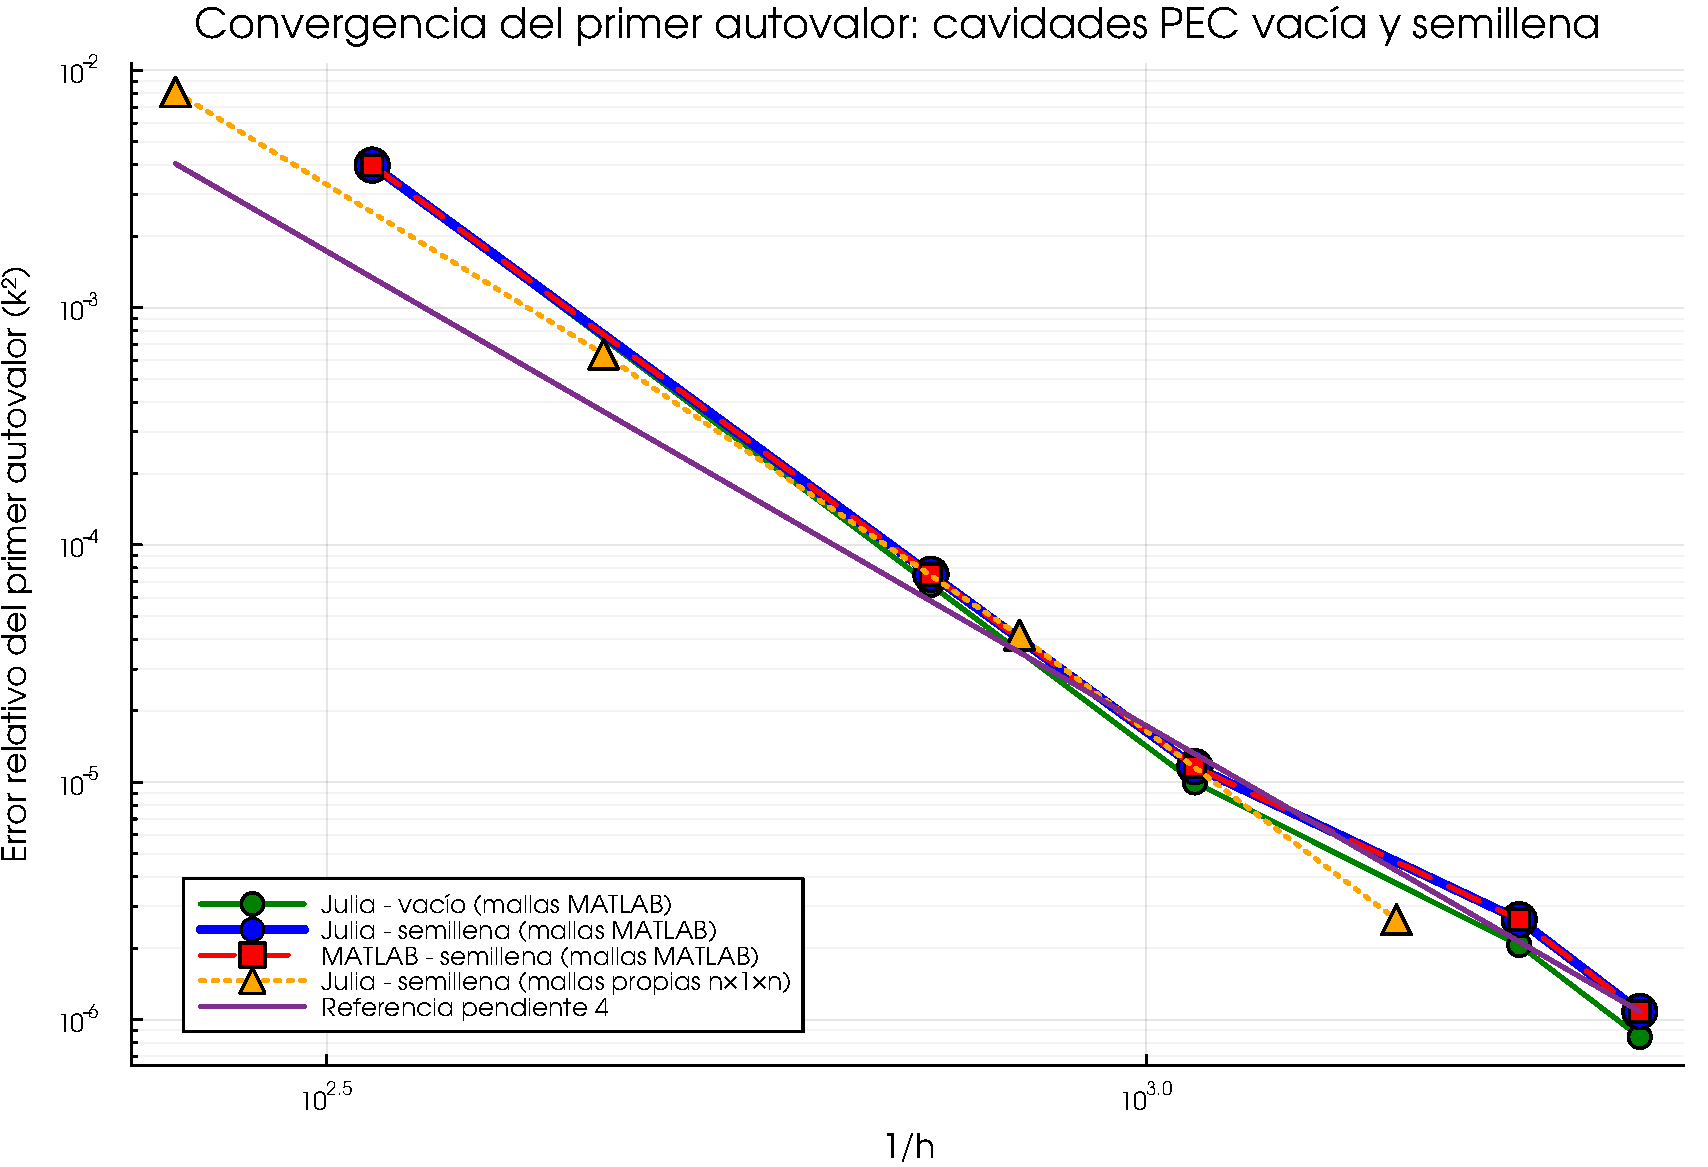
\includegraphics[width=\textwidth]{figuras/convergencia_combinada_cavidades.pdf}%
      }{%
        \centering\footnotesize\itshape
        [figura: convergencia\_combinada\_cavidades.pdf]%
      }
    \end{column}
  \end{columns}
\end{frame}

%--------------------------------------------------------------------------
% DIAPOSITIVA 22 — RENDIMIENTO JULIA vs MATLAB
%--------------------------------------------------------------------------
\begin{frame}{Rendimiento: Julia vs MATLAB}
  \begin{center}
  \footnotesize
  \begin{tabular}{lrrr}
    \toprule
    \textbf{Etapa} & \textbf{MATLAB} & \textbf{Julia} & \textbf{Speedup} \\
    \midrule
    Generación de coeficientes & 251 ms      & 4.5 ms      & \textbf{56$\times$} \\
    Numeración de DOFs         & 28.3 ms     & 1.0 ms      & \textbf{30$\times$} \\
    Ensamblado + Dirichlet     & 17136.7 ms  & 1199.4 ms   & \textbf{14$\times$} \\
    Solver                     & 424.2 ms    & 391.8 ms    & 1.1$\times$ \\
    \bottomrule
  \end{tabular}
  \end{center}

  \vspace{3mm}
  \begin{itemize}
    \item Memoria: bloque free-free idéntico (25.2 MB, malla 5)
    \item Profiling: \texttt{stiff\_matrix\_element} (823 llamadas, 926808 allocs),
          \texttt{mass\_matrix\_element} (589 llamadas, 915800 allocs)
  \end{itemize}
\end{frame}

%==========================================================================
\section{Aplicación real}
%==========================================================================

%--------------------------------------------------------------------------
% DIAPOSITIVA 24 — GUÍA DE ONDA CON CONDICIÓN PEC
%--------------------------------------------------------------------------
\begin{frame}{Aplicación: guía de onda con condición PEC}
  \begin{columns}[T]
    \begin{column}{0.52\textwidth}
      \begin{itemize}
        \item Geometría real mallada con Gmsh
        \item Cálculo de los modos de resonancia
        \item Comparación con la solución analítica de la guía
        \item Visualización de los modos (Manim)
        \item Verificación de ausencia de modos espurios
      \end{itemize}
    \end{column}
    \begin{column}{0.46\textwidth}
      \IfFileExists{imagenes/guia_onda_pec.png}{%
        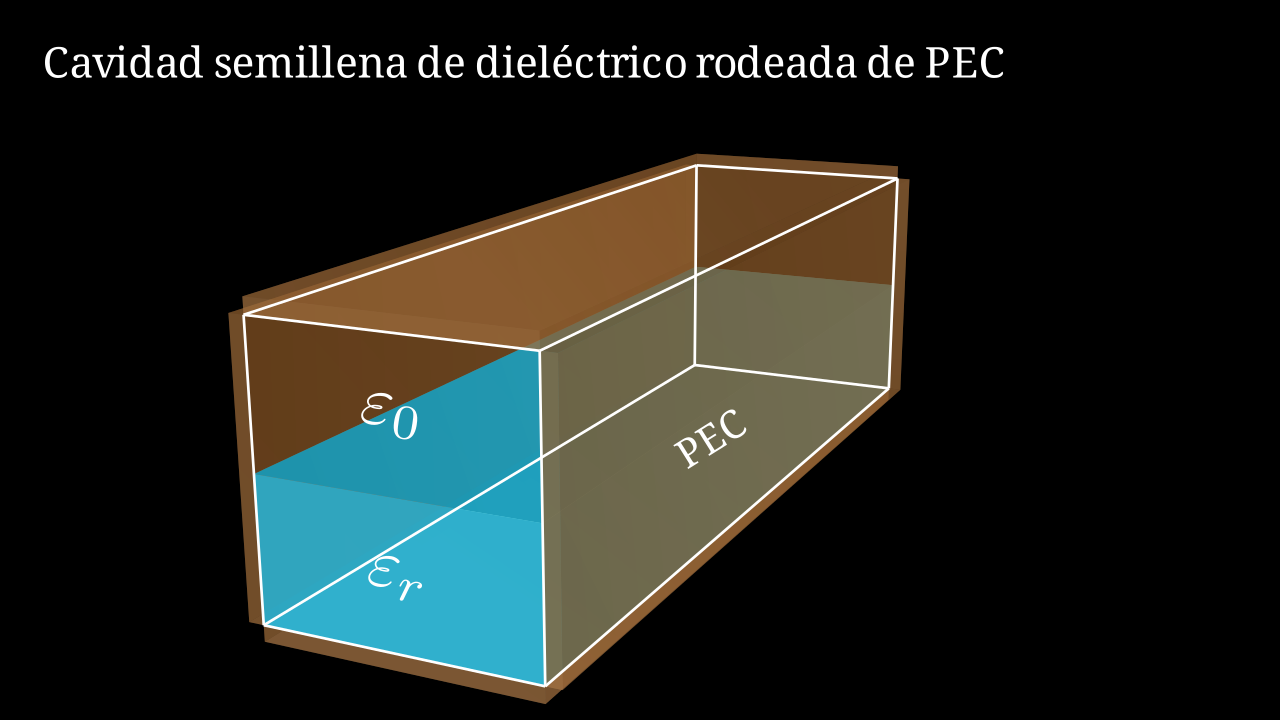
\includegraphics[width=\textwidth]{imagenes/guia_onda_pec.png}%
      }{%
        \centering\footnotesize\itshape
        [figura: guia\_onda\_pec.png]%
      }
    \end{column}
  \end{columns}
\end{frame}

%==========================================================================
\section{Conclusiones}
%==========================================================================

%--------------------------------------------------------------------------
% DIAPOSITIVA 26 — CONCLUSIONES
%--------------------------------------------------------------------------
\begin{frame}{Conclusiones}
  \textbf{Objetivos cumplidos:}
  \begin{itemize}
    \item Elemento implementado y verificado contra el artículo
    \item Coeficientes reproducen la Tabla II (2916 entradas)
    \item Convergencia $O(h^4)$ confirmada en cavidad llena y semillena
    \item Rendimiento superior a MATLAB (hasta $56\times$ en generación de
          coeficientes)
    \item Paquete modular, documentado y con tests automatizados
  \end{itemize}

  \vspace{2mm}
  \textbf{Impacto:}
  \begin{itemize}
    \item Accesibilidad educativa (Julia, código abierto)
    \item Base para futuras extensiones a orden superior
    \item Contribución a la línea de investigación de GREMA
  \end{itemize}

  \vspace{2mm}
  \textbf{Trabajo futuro:}
  \begin{itemize}
    \item Optimizar el ensamblado (reducir asignaciones)
    \item Extender a elementos de orden superior
    \item Integración con HOFEM
  \end{itemize}
\end{frame}

%--------------------------------------------------------------------------
% DIAPOSITIVA 27 — AGRADECIMIENTOS / CIERRE
%--------------------------------------------------------------------------
\begin{frame}
  \centering
  \Huge \textcolor{azulUC3M}{¡Gracias!}
  \vspace{8mm}

  \normalsize
  Preguntas

  \vspace{4mm}
  \footnotesize\color{grisUC3M}
  Datos de contacto / repositorio
\end{frame}

%==========================================================================
% APÉNDICES (diapositivas de reserva para el turno de preguntas)
%==========================================================================
\appendix

%--------------------------------------------------------------------------
% APÉNDICE A — ESPACIO H2 Y MONOMIOS
%--------------------------------------------------------------------------
\begin{frame}{Apéndice A: Espacio $H_2$ y monomios}
  \begin{itemize}
    \item Definición de $Q_{p_1,p_2,p_3}$
    \item Los 54 monomios del espacio mixto
    \item Correspondencia monomio $\leftrightarrow$ grado de libertad
  \end{itemize}
\end{frame}

%--------------------------------------------------------------------------
% APÉNDICE B — MATRIZ DE MOMENTOS G
%--------------------------------------------------------------------------
\begin{frame}{Apéndice B: Matriz de momentos $G$}
  \begin{itemize}
    \item Construcción de $G$ a partir de los funcionales de momento
    \item Estructura por bloques (aristas, caras, volumen)
    \item Inversión exacta con coeficientes enteros
  \end{itemize}
\end{frame}

%--------------------------------------------------------------------------
% APÉNDICE C — TRANSFORMACIONES DE PIOLA
%--------------------------------------------------------------------------
\begin{frame}{Apéndice C: Transformaciones de Piola}
  \begin{itemize}
    \item Piola covariante:
      \begin{equation*}
        \mathbf{v} = J^{-T}\, \hat{\mathbf{v}}
      \end{equation*}
    \item Piola contravariante:
      \begin{equation*}
        \mathbf{w} = \frac{1}{\det J}\, J\, \hat{\mathbf{w}}
      \end{equation*}
    \item Garantía de continuidad tangencial en $H(\mathrm{curl})$
  \end{itemize}
\end{frame}

%--------------------------------------------------------------------------
% APÉNDICE D — PERMUTACIÓN DE NODOS DE GMSH
%--------------------------------------------------------------------------
\begin{frame}{Apéndice D: Permutación de nodos de Gmsh}
  \begin{itemize}
    \item Orden de Gmsh vs orden del elemento
    \item Permutación aplicada:
      \begin{center}
        \texttt{[3, 7, 8, 4, 2, 6, 5, 1]}
      \end{center}
    \item Test específico: \texttt{test\_06\_gmsh\_node\_order.jl}
  \end{itemize}
\end{frame}

%--------------------------------------------------------------------------
% APÉNDICE E — ETIQUETAS DE MALLA
%--------------------------------------------------------------------------
\begin{frame}{Apéndice E: Etiquetas de malla}
  \begin{itemize}
    \item Uso de etiquetas PolyFace/Solid de Gmsh
    \item Ventaja frente a inferir geometría por coordenadas
    \item Test: \texttt{test\_09\_tags.jl}
  \end{itemize}
\end{frame}

%--------------------------------------------------------------------------
% APÉNDICE F — CUADRATURA DE GAUSS-LEGENDRE
%--------------------------------------------------------------------------
\begin{frame}{Apéndice F: Cuadratura de Gauss-Legendre}
  \begin{itemize}
    \item Puntos y pesos de Gauss-Legendre
    \item Orden de cuadratura suficiente para integrandos de grado 4
    \item Test: \texttt{test\_01\_quadrature.jl}
  \end{itemize}
\end{frame}

%--------------------------------------------------------------------------
% APÉNDICE G — SOLVER DE AUTOVALORES
%--------------------------------------------------------------------------
\begin{frame}{Apéndice G: Solver de autovalores}
  \begin{itemize}
    \item Problema generalizado $K g = \lambda M g$
    \item Shift-invert con Arpack
    \item Solver denso para mallas pequeñas
    \item Criterio de selección
  \end{itemize}
\end{frame}

%--------------------------------------------------------------------------
% APÉNDICE H — RESULTADOS COMPLETOS DE CONVERGENCIA
%--------------------------------------------------------------------------
\begin{frame}{Apéndice H: Resultados completos de convergencia}
  \begin{itemize}
    \item Tabla completa de errores por malla
    \item Ajuste log-log y pendientes
    \item Comparación con el orden teórico
  \end{itemize}
\end{frame}

%--------------------------------------------------------------------------
% APÉNDICE I — CÓDIGO DE EJEMPLO
%--------------------------------------------------------------------------
\begin{frame}[fragile]{Apéndice I: Código de ejemplo}
  \begin{lstlisting}[language=Julia]
using NedelecHex

mesh = read_mesh("cavity.msh")
K, M = assemble(mesh)
lambda = solve_eigen(K, M, nev=10)
  \end{lstlisting}
\end{frame}

%==========================================================================
\end{document}
%==========================================================================
